\chapter{Implementation Documentation}
Detailed description of \textbf{database} and \textbf{backend components and functions}.  

\section{Database design}
For this purpose well defined database is a necessity. In this chapter we learn how the proposed objects are represented how relations between these objects are maintaned and what information tables exist.
\subsection{Schema}
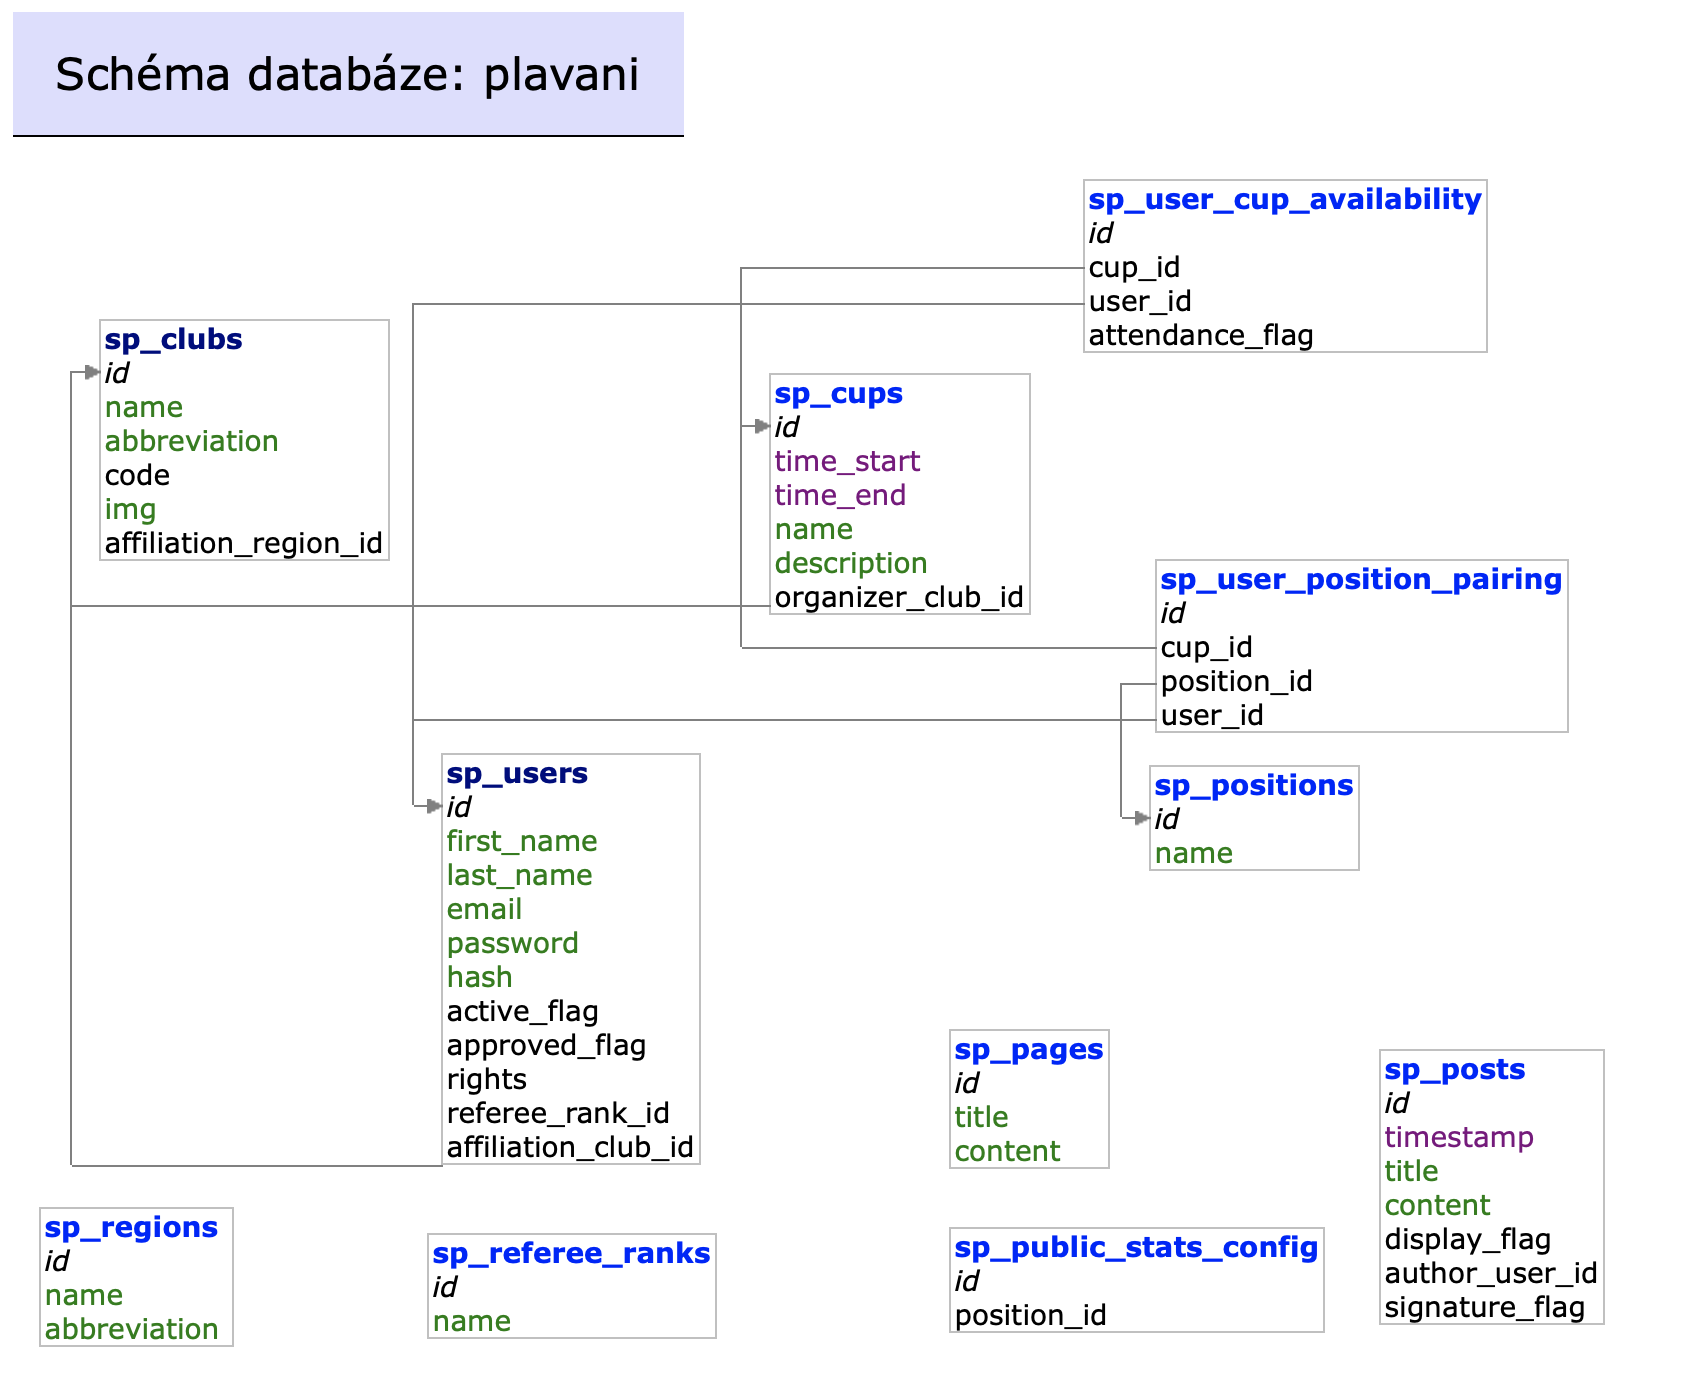
\includegraphics[scale=0.45]{img/schema.png}
\subsection{Object tables}
These are the tables in database modeling the object to satisfy the primary motivation defined as the \textbf{problem paradigm}. These rows are then being converted to Objects and returned to user by appropriate Manager.
% \newline
\subsubsection*{sp\_posts}
Posts for main page are stored in this table.
\newline
\underline{Table preview}
\begin{center}
  \begin{tabular}{||c c c c c c c||} 
  \hline
  id & timestamp & title & content & display\_flag & author & sign\_flag  \\ [0.5ex] 
  \hline\hline
  1 & 2018-01-... & New Por... & SwimmPair... & 1 & 21 & 0 \\ 
  \hline
  2 & 2018-03-...  & Updates & This web... & 1 & 21 & 0 \\ 
 \hline
  ... & ... & ... & ... & ... & ...  & ... \\ [0.5ex] 
  \hline
  \end{tabular}
\end{center}
\underline{Columns description}
\begin{enumerate}
  \setlength\itemsep{0em}
  \item \textbf{id}, PK, int(11), AUTOINCREMENT
  \item \textbf{timestamp}, datetime
  \item \textbf{title}, text
  \item \textbf{content}, text
  \item \textbf{display\_flag}, tinyint
  \item \textbf{author}, FK, int(11) $|$ NULL
  \item \textbf{sign\_flag}, tinyint
\end{enumerate}

\subsubsection*{sp\_users}
Users are stored in this table.
\newline
\underline{Table preview}
\begin{center}
  \begin{tabular}{||c c c c c c c||} 
  \hline
  id & first\_name & last\_name & email & password & hash & ... \\ [0.5ex] 
  \hline\hline
  1 & Lukáš & Kousal & lukas@swim.cz & -PASS- & -HASH- & ... \\ 
  \hline
  ... & ... & ... & ... & ... & ... & ... \\
  \hline
  N & ... & ... & ... & ... & ... & ... \\ 
  \hline
 \end{tabular}
 \end{center}
 \underline{Columns description}
 \begin{enumerate}
   \setlength\itemsep{0em}
   \item \textbf{id}, PK, int(11), AUTOINCREMENT
   \item \textbf{first\_name}, varchar(50)
   \item \textbf{last\_name}, varchar(50)
   \item \textbf{email}, varchar(100) //unique identifier
   \item \textbf{password}, varchar(100)
   \item \textbf{hash}, varchar(32)
   \item \textbf{active}, tinyint(1)
   \item \textbf{approved}, tinyint(1)
   \item \textbf{rights}, int(11)
   \item \textbf{klubaffil}, FK, int(11)
\end{enumerate}

\subsubsection*{sp\_clubs}
Clubs are stored in this table. 
\newline
\underline{Table preview}
\begin{center}
 \begin{tabular}{||c c c c c||} 
 \hline
 id & name & zkratka & idklubu & img \\ [0.5ex] 
 \hline\hline
 1 & Klub plaveckých sportů Vyškov & KPSVy & 614 & null.jpg \\  
 \hline
 ... & ... & ... & ... & ... \\ [0.5ex]
\hline
 14 & TJ Rožnov pod Radhoštěm & TJRo & 0 & null.jpg \\
 \hline
\end{tabular}
\end{center}
\underline{Columns description}
\begin{enumerate}
  \setlength\itemsep{0em}
  \item \textbf{id}, PK , int(11), AUTOINCREMENT
  \item \textbf{name}, varchar(512)
  \item \textbf{zkratka}, text
  \item \textbf{idklubu}, int(11)
  \item \textbf{img}, text
\end{enumerate}

\subsubsection*{sp\_cups}
Cups are stored in this table.
\newline
\underline{Table preview}
\begin{center}
 \begin{tabular}{||c c c c c||} 
 \hline
 id & date & name & description & owningclub  \\ [0.5ex] 
 \hline\hline
 1 & 2017-06-12 & GJW Cup I. & Cup organized by GJW PV, ... & 2 \\ 
 \hline
 ... & ... & ... & ... & ...  \\ [0.5ex] 
 \hline
\end{tabular}
\end{center}
\underline{Columns description}
\begin{enumerate}
  \setlength\itemsep{0em}
  \item \textbf{id}, PK , int(11), AUTOINCREMENT
  \item \textbf{date}, date
  \item \textbf{name}, text
  \item \textbf{description}, text
  \item \textbf{owningclub}, int(11)
\end{enumerate}


\subsubsection*{sp\_positions}
List of Positions for which we are pairing users are stored here.
\newline
\underline{Table preview}
\begin{center}
 \begin{tabular}{||c c||} 
 \hline
 id & poz  \\ [0.5ex] 
 \hline\hline
 1 & Vrchní rozhodčí \\ 
 \hline
 ... & ...  \\ [0.5ex]
\hline
 19 & Ostatní  \\
 \hline
\end{tabular}
\end{center}
\underline{Columns description}
\begin{enumerate}
  \setlength\itemsep{0em}
  \item \textbf{id}, PK , int(11), AUTOINCREMENT
  \item \textbf{poz}, varchar(512)
\end{enumerate}

\subsection{Relation tables}
Relation tables hold the most important information stored in the SwimmPair system - the \textbf{pairings} and \textbf{data for underlying statistics}. Both availability for cups and pairings to positions are represented here.
\subsubsection*{sp\_cup\_user\_availability}
This table stores relationships between referees/\underline{users} and \underline{cups} called availability. Referees are signed up by their team manager or themselves as available for the cup. In case of sudden inability to participate, the attendance\_flag is switched to 0 in case the user is already assigned to some position. In that case the administrator is going to see the user in red box.
\newline
\underline{Table preview}
\begin{center}
 \begin{tabular}{||c c c c||} 
 \hline
 id & cup\_id & user\_id & attendance\_flag  \\ [0.5ex] 
 \hline\hline
 1 & 3 & 21 & 1 \\ 
 \hline
 2 & 3 & 1 & 1 \\ 
 \hline
 7 & 3 & 19 & 0 \\ 
 \hline
 ... & ... & ... & ...  \\ [0.5ex] 
 \hline
\end{tabular}
\end{center}
\underline{Columns description}
\begin{enumerate}
  \setlength\itemsep{0em}
  \item \textbf{id}, PK, int(11), AUTOINCREMENT
  \item \textbf{cup\_id}, FK, int(11)
  \item \textbf{user\_id}, int(11)
  \item \textbf{attendance\_flag}, tinyint(1)
\end{enumerate}

\subsubsection*{sp\_position\_user\_pairing}
This table stores pairing information about available referees/users on positions for each cup. This is the most time saving utility of the SwimmPair.
\newline
\underline{Table preview}
\begin{center}
 \begin{tabular}{||c c c c||} 
 \hline
 id & cup\_id & position\_id & user\_id  \\ [0.5ex] 
 \hline\hline
 46 & 5 & 5 & 21 \\ 
 \hline
 484 & 3 & 1 & 21 \\ 
 \hline
 485 & 3 & 1 & 22 \\ 
 \hline
 486 & 3 & 2 & 7 \\
 \hline
 487 & 3 & 3 & 15 \\
 \hline
 487 & 3 & 5 & 12 \\
 \hline
 487 & 3 & 7 & 14 \\
 \hline
 ... & ... & ... & ... \\ [0.5ex] 
 \hline
\end{tabular}
\end{center}
\underline{Columns description}
\begin{enumerate}
  \setlength\itemsep{0em}
  \item \textbf{id}, PK, bigint(11), AUTOINCREMENT
  \item \textbf{cup\_id}, FK, int(11)
  \item \textbf{position\_id}, FK, int(11)
  \item \textbf{user\_id}, FK, int(11)
\end{enumerate}
\subsection{Content adjustment tables}
\subsubsection*{sp\_public\_stats\_config}
Configuration table of which positions in what order should be displayed in statistics on frontend. For frontend then LEFT-JOIN \textbf{position\_id} from table \textbf{sp\_positions} ON \textbf{id} and display \textbf{poz}.
\newline
\underline{Table preview}
\begin{center}
 \begin{tabular}{||c c||} 
 \hline
 id & position\_id  \\ [0.5ex] 
 \hline\hline
 148 & 1 \\ 
 \hline
 149 & 8  \\ 
 \hline
 150 & 2  \\ 
 \hline
 151 & 4  \\ 
 \hline
 152 & 6  \\  
 \hline
 \end{tabular}
\end{center}
\underline{Columns description}
\begin{enumerate}
  \setlength\itemsep{0em}
  \item \textbf{id}, PK, int(11), AUTOINCREMENT
  \item \textbf{position\_id}, FK, int(11)
\end{enumerate}

\subsubsection*{sp\_pages}
SwimmPair static Pages.
\newline
\underline{Table preview}
\begin{center}
 \begin{tabular}{||c c c||} 
 \hline
 id & title & content \\ [0.5ex] 
 \hline\hline
 1 & Kontakty &  \textless h1\textgreater Title\textless /h1\textgreater  \textless p\textgreater Contact information +420...\textless /p\textgreater  \\

 \hline
\end{tabular}
\end{center}
\underline{Columns description}
\begin{enumerate}
  \setlength\itemsep{0em}
  \item \textbf{id}, PK , int(11), AUTOINCREMENT
  \item \textbf{title}, text
  \item \textbf{content}, text
\end{enumerate}
\newpage
\section{Managers documentation}
\par These five controllers work with objects and provide login (i.e. joining more tables in varios ways to achieve all functionality).
\subsection{PostsManager.php}
\begin{itemize}
  \setlength\itemsep{0em}
  \item \underline{Post} $\vert$ null $\leftarrow$ \textbf{GetPostById}(\$id)
  \newline    $\searrow$ \_CreatePostOrNullFromStatement(\$stmt)
  \newline    $\searrow$ \_CreatePostFromRow(\$row)
  \item \underline{Post[]} $\vert$ null $\leftarrow$ \textbf{GetLastThreePosts}()
  \newline    $\searrow$ \_CreatePostsFromStatement(\$stmt)
  \newline    $\searrow$ \_CreatePostFromRow(\$row)
  \item \underline{Post[]} $\vert$ null $\leftarrow$ \textbf{GetLastNPosts}(\$N)
  \newline    $\searrow$ \_CreatePostsFromStatement()
  \newline    $\searrow$ \_CreatePostFromRow(\$row)
  \item \underline{true} $\vert$ false $\leftarrow$ \textbf{AddNewPost}(\$title, \$content)
  \item \underline{Post[]} $\vert$ false $\leftarrow$ \textbf{FindAllPostsOrderedByIdDesc}()
  \newline    $\searrow$ \_CreatePostsFromStatement(\$stmt)
  \newline    $\searrow$ \_CreatePostFromRow(\$row)
  \item \underline{true} $\vert$ false $\leftarrow$ \textbf{UpdatePost}(\$id, \$title, \$article)
\end{itemize}
\subsection{UsersManager.php}
\begin{itemize}
  \setlength\itemsep{0em}
  \item \underline{User} $\vert$ null $\leftarrow$ \textbf{GetUserById}(\$id)
  \newline    $\searrow$ \_CreateUserOrNullFromStatement(\$stmt)
  \newline    $\searrow$ \_CreateUserFromRow(\$row)
  \item \underline{User[]} $\vert$ null $\leftarrow$ \textbf{FindAllActiveUsersOrderByLastNameDesc}()
  \newline    $\searrow$ \_CreateUsersFromStatement(\$stmt)
  \newline    $\hookrightarrow$ \_CreateUserFromRow (\$row)
  \item \underline{User[]} $\vert$ null $\leftarrow$ \textbf{FindAllInactiveUsersOrderByLastNameDesc}()
  \newline    $\searrow$ \_CreateUsersFromStatement(\$stmt)
  \newline    $\hookrightarrow$ \_CreateUserFromRow (\$row)
  \item \underline{User[]} $\vert$ null $\leftarrow$ \textbf{FindAllRegisteredMatesForTheCup}(\$cupId, \$teamId)
  \newline    $\searrow$ \_CreateUsersFromStatement(\$stmt)
  \newline    $\hookrightarrow$ \_CreateUserFromRow (\$row)
  \item \underline{User[]} $\vert$ null $\leftarrow$ \textbf{FindAllMates}(\$teamId)
  \newline    $\searrow$ \_CreateUsersFromStatement(\$stmt)
  \newline    $\hookrightarrow$ \_CreateUserFromRow(\$row)
  \item \underline{User[]} $\vert$ null $\leftarrow$ \textbf{FindAllRegisteredUsersForTheCup}(\$cupId)
  \newline    $\searrow$ \_CreateUsersFromStatement(\$stmt)
  \newline    $\hookrightarrow$ \_CreateUserFromRow(\$row)
  \item \underline{User[]} $\vert$ null $\leftarrow$ \textbf{FindAllNametagsForTheCup}(\$cupId)
  \newline    $\searrow$ \_CreateUsersFromStatement(\$stmt)
  \newline    $\hookrightarrow$ \_CreateUserFromRow(\$row)
  \item \underline{User[]} $\vert$ null $\leftarrow$ \textbf{FindPairedUsersOnCupForPosition}(\$cupId, \$posId)
  \newline    $\searrow$ \_CreateUsersFromStatement(\$stmt)
  \newline    $\hookrightarrow$ \_CreateUserFromRow(\$row)
  \item \underline{Pair[]} $\vert$ null $\leftarrow$ \textbf{FindPairedPozIdUserIdOnCup}(\$cupId)
  \newline    $\searrow$ \_CreatePairsFromStatement(\$stmt)
  \newline    $\hookrightarrow$ \_CreatePairFromRow(\$row)
  \item \underline{string} $\vert$ null $\leftarrow$ \textbf{GetClubAbbreviationByAffiliationId}(\$id)
  \newline    $\searrow$ \_GetSingleResultFromStatement(\$stmt)
  \item \underline{string} $\vert$ null $\leftarrow$ \textbf{GetUserFullNameById}(\$id)
  \newline    $\searrow$ \_GetSingleResultFromTwoColsStatement(\$stmt)
  \item \underline{true} $\vert$ \underline{false} $\leftarrow$ \textbf{UserWithEmailExists}(\$email)
  \item \underline{true} $\vert$ false $\leftarrow$ \textbf{RegisterUserFromAdmin}(\$first\_name, \$last\_name,
  \newline    \$email, \$password, \$rights, \$klubaffil)
  \item \underline{true} $\vert$ false $\leftarrow$ \textbf{SendYouWereRegisteredFromAdmin}(\$email,
  \newline    \$password)
  \item \underline{true} $\vert$ false $\leftarrow$ \textbf{ApproveUser}(\$userId)
  \item \underline{true} $\vert$ false $\leftarrow$ \textbf{UpdatePairing}(\$JSON)
\end{itemize}
\subsection{ClubsManager.php}
\begin{itemize}
  \setlength\itemsep{0em}
  \item \underline{Club} $\vert$ null $\leftarrow$ \textbf{GetClubById}(\$id)
  \newline    $\searrow$ \_CreateClubFromStatement(\$stmt)
  \newline    $\searrow$ \_CreateClubFromRow(\$row)
  \item \underline{Club[]} $\vert$ null $\leftarrow$ \textbf{FindAllClubs}()
  \newline    $\searrow$ \_CreateClubsFromStatement(\$stmt)
  \newline    $\hookrightarrow$ \_CreateClubFromRow(\$row)
\end{itemize}
\subsection{CupsManager.php}
\begin{itemize}
  \setlength\itemsep{0em}
  \item \underline{Cup[]} $\vert$ null $\leftarrow$ \textbf{FindAllUpcomingCupsEarliestFirst}()
  \newline    $\searrow$ \_CreateCupsFromStatement(\$stmt)
  \newline    $\hookrightarrow$ \_CreateCupFromRow(\$row)
  \item \underline{Cup[]} $\vert$ null $\leftarrow$ \textbf{FindAllPastCupsMostRecentFirst}()
  \newline    $\searrow$ \_CreateCupsFromStatement(\$stmt)
  \newline    $\hookrightarrow$ \_CreateCupFromRow(\$row)
  \item \underline{string} $\vert$ null  $\leftarrow$ \textbf{GetCupNameById}(\$id)
  \newline    $\searrow$ \_GetSingleResultFromStatement(\$stmt)
  \newline    $\searrow$ \_GetSingleResultFromStatement (\$stmt)
  \item \underline{Cup} $\vert$ null  $\leftarrow$  \textbf{GetCupById}(\$id)
  \newline    $\searrow$ \_CreateCupOrNullFromStatement(\$stmt)
  \newline    $\searrow$ \_CreateCupFromRow(\$row)
  \item \underline{Pair[]} $\vert$ null $\leftarrow$  \textbf{FindPairingsForThisCup}(\$id)
  \newline    $\searrow$ \_CreatePairsFromStatement(\$stmt)
  \newline    $\hookrightarrow$ \_CreatePairFromRow(\$row)
  \item \underline{true} $\vert$ false $\leftarrow$  \textbf{InsertNewCupFromAdmin}(\$name, \$date, \$club,
  \newline    \$content)
  \item \underline{true} $\vert$ \underline{false} $\leftarrow$  \textbf{IsUserAvailableForTheCup}(\$userId, \$cupId)
  \item \underline{true} $\vert$ false $\leftarrow$  \textbf{UpdatePairingForThisCup}(\$cupId, \$JSON)
  \item \underline{true} $\vert$ false $\leftarrow$  \textbf{UpdateAvailabilityForThisCup}(\$cupId, \$JSON)
  \item \underline{true} $\vert$ false $\leftarrow$  \textbf{AddAvailableUserForTheCup}(\$cupId, \$userId)
\end{itemize}
\subsection{PositionsManager.php}
\begin{itemize}
  \setlength\itemsep{0em}
  \item \underline{Position[]} $\vert$ null $\leftarrow$  \textbf{FindAllPositions}()
  \newline    $\searrow$ \_CreatePositionsFromStatement(\$stmt)
  \newline    $\hookrightarrow$ \_CreatePositionFromRow(\$row)
  \item \underline{string} $\vert$ null $\leftarrow$ \textbf{GetPositionNameById}(\$id)
  \newline    $\searrow$ \_GetSingleResultFromStatement(\$stmt)
\end{itemize}

\section{Application structure - PHP files defined}
\subsection*{User part of the system}
The system is running on Czech URLs for convinience reasons of browsing. English equivalents of route pages are attached in brackets to demonstrate what the pages do for non-czech speaker. There is no client side routing with traditional LAMP stack.
\newline
\begin{forest}
  for tree={
    font=\ttfamily,
    grow'=0,
    child anchor=west,
    parent anchor=south,
    anchor=west,
    calign=first,
    edge path={
      \noexpand\path [draw, \forestoption{edge}]
      (!u.south west) +(7.5pt,0) |- node[fill,inner sep=1.25pt] {} (.child anchor)\forestoption{edge label};
    },
    before typesetting nodes={
      if n=1
        {insert before={[,phantom]}}
        {}
    },
    fit=band,
    before computing xy={l=15pt},
  }
[www.SwimmPair.cz/index.php
  [Zavody (Cups)
    [nadchazejici.php (upcoming.php)
      [zavod.php (cup.php)]
    ]
    [archiv.php (archive.php)
      [zavod.php (cup.php)] 
    ]
  ]
  [Rozhodci (Referees)
    [lide.php (users.php)
      [clovek.php (user.php)]
    ]
    [kluby.php (clubs.php)
      [klub.php (club.php)]
    ]
  ]
  [/pravidla/index.php (/rules/index.php)]
  [kontakty.php (contacts.php)]
  [/admin/index.php]
]
\end{forest}
\newpage
\subsection*{Administrative part of the system} 
The administration has following structure. After going to /admin/index.php user gets logs in and goes to /administration/profile.php. Regarding user's rights (that are passed around along with other information in \textbf{SESSION}, retrievable like \textbf{\$SESSION\_['rights']}) one has following structure (\textbf{Administration}, \textbf{My Club}, \textbf{Me}). Each user has profile settings for reseting password and other stuff.  
\newline
\begin{forest}
  for tree={
    font=\ttfamily,
    grow'=0,
    child anchor=west,
    parent anchor=south,
    anchor=west,
    calign=first,
    edge path={
      \noexpand\path [draw, \forestoption{edge}]
      (!u.south west) +(7.5pt,0) |- node[fill,inner sep=1.25pt] {} (.child anchor)\forestoption{edge label};
    },
    before typesetting nodes={
      if n=1
        {insert before={[,phantom]}}
        {}
    },
    fit=band,
    before computing xy={l=15pt},
  }
[www.SwimmPair.cz/administration/profile.php
  [pridat\_aktualitu.php (add\_post.php)]
  [editovat\_aktuality.php (edit\_posts.php)
    [editovat\_aktualitu.php (edit\_post.php)]
  ]
  [nove\_registrovani.php (newly\_registered.php)]
  [rozhodci\_zavody.php (referees\_cups.php)
    [pairing.php (pairing.php)]
  ]
  [zaregistrovat\_uzivatele.php (register\_user.php)]
  [editovat\_profily.php (edit\_profiles.php)
    [editovat\_profil.php (edit\_profile.php)]
  ]
  [novy\_klub.php (add\_club.php)]
  [sprava\_klubu.php (edit\_clubs.php)
    [editovat\_klub.php (edit\_club.php)]
  ]
  [novy\_kraj.php (new\_region.php)]
  [sprava\_kraju.php (edit\_regions.php)
    [editovat\_kraj.php (edit\_region.php)]
  ]
  [konfigurace\_statistik.php (configure\_stats.php)]
  [editovat\_stranku.php (edit\_page.php)]
]
\end{forest}
\newline
\begin{forest}
  for tree={
    font=\ttfamily,
    grow'=0,
    child anchor=west,
    parent anchor=south,
    anchor=west,
    calign=first,
    edge path={
      \noexpand\path [draw, \forestoption{edge}]
      (!u.south west) +(7.5pt,0) |- node[fill,inner sep=1.25pt] {} (.child anchor)\forestoption{edge label};
    },
    before typesetting nodes={
      if n=1
        {insert before={[,phantom]}}
        {}
    },
    fit=band,
    before computing xy={l=15pt},
  }
[My Club
  [pridat\_zavod.php (add\_cup.php)]
  [prihlasit\_moje\_lidi.php (sign\_availability\_mates.php)
    [prihlasit\_moje\_lidi\_na.php (sign\_availability\_mates\_for.php)]
  ]
]
\end{forest}
\newline
\begin{forest}
  for tree={
    font=\ttfamily,
    grow'=0,
    child anchor=west,
    parent anchor=south,
    anchor=west,
    calign=first,
    edge path={
      \noexpand\path [draw, \forestoption{edge}]
      (!u.south west) +(7.5pt,0) |- node[fill,inner sep=1.25pt] {} (.child anchor)\forestoption{edge label};
    },
    before typesetting nodes={
      if n=1
        {insert before={[,phantom]}}
        {}
    },
    fit=band,
    before computing xy={l=15pt},
  }
[Me
  [sebe\_na\_zavod.php (myself\_for\_cup.php)
    [prihlasit\_se\_na.php (sign\_myself\_for.php)]
  ]
]
\end{forest}
\newline
\section{JavaScript functions documentation}
Several features of public website implemented in JavaScript for interactive browsing are described here.
\subsection*{Library js/SwimmPairFrontendJSLib.js}
This library is created to support Ajax calls and DOM operations on frontend.
\newline 
GetPostAppendPost(PushLastId()) -- ConstructNextPost
\newline
ProcessClubForTheSeason(clubId, this) -- CommunicateClubStatsXhrAndUpdateTable(clubId, year) -- UpdateClubStatsTable(returnedJSON)
\newline
\subsection*{XMLHttpRequest endpoints}
\begin{itemize}
    \item get\_post\_following.php, \textbf{GET args}: \textbf{id}
    \item get\_person\_statistics\_for\_the\_season.php, \textbf{GET args}: user\textunderscore \textbf{id}, year
    \item get\_club\_statistics\_for\_the\_season.php, \textbf{GET args}: club\textunderscore \textbf{id}, year
\end{itemize}
\subsection{Previous post}
This button on the main page serves as a tool for loading next post. This button has \textbf{onclick="GetPostAppendPost(PushLastId())"}. These are both JavaScript functions, \textbf{PushLastId()} detects id \textbf{\textless article class="post" id="X"... } of last article class="post" from DOM by querySelector and returns it. This value is then used as an argument of call \textbf{GetPostAppendPost(id)}. This function requests article by GET request \textbf{XMLHttpRequest/get\_following\_post.php?id=X}.  
If the result is
\newline i)  \textbf{null} button is deleted since there are no other articles to pull from DB,
\newline ii) \textbf{post} next article is constructed and appended from response.
\subsection{User statistics - year change}
All individual referees have seasons years picker when opened. Default season is the current season. Clicking different season visibily changes selected year and obtains appropriate statistics and updates the stats table. Clicking \textbf{\textless span onclick="ProcessPersonForTheSeason(userId, this)"... } calls inside \textbf{CommunicateStatsXhrAndPopulateStats(userId, year)} gets data from \textbf{XMLHttpRequest/call\_get\_person\_statistics\_for\_the\_season.php}\newline \textbf{?id=userId\&year=YYYY} and updates table. Also via \text{this} reference in call the button is marked as selected.  
\subsection{Club statistics - year change}
Club statistics are updated by clicking appropriate year that gets switched. Year onclick calls \textbf{ProcessClubForTheSeason(clubId, this)} which gets statistics by calling \textbf{CommunicateClubStatsXhrAndUpdateTable(clubId, year)}
\newline by calling \textbf{XMLHttpRequest/get\_club\_statistics\_for\_the\_season.php}
\newline \textbf{?id=clubId\&year=Year} and subsequently calling
\newline \textbf{UpdateClubStatsTable(returnedGetJSON)} which literally updates stats.
\subsection{Filtering referees}
This function is triggered by one of these: KrajPickerTapped(this), TridaPickerTapped(this) or SearchPerformed(). Each one calls FilterRozhodci("kraje", "tridy", "inputTrida", "nopplfound"). We then loop all people visible/hidden and check if this one's Region IsPermissible(args[]), then if one's Class IsPermissible(args[]) and then if one's IsNamePermissible(args[]). We then set one element style to style="" and continue cycle execution. If we fail one of these three conditions we proceed to code below which sets element style to style="display:none". After the cycle when check the aux variable and if our query is indeed empty we write it for the user.
\par
This long procedure gets triggered and subsequently executed everytime region, class or name is changed. Performance should be fine here since the algorithm is dependent on human input. 
